\chapter{Convolution Demonstration}
% Authors: Mimee Xu , Sai Anirudh Kondaveeti, Rui Jiang(rj1407), 2/20/18.
\section{Natural Signal Patterns}
Neural networks can be used to model audio, image, text, or other signals. The signals are represented as sequences of scalars. Audio is often represented as waveform heights, images are often represented as pixel values, and text is often represented as one hot vectors.

Natural signals (not artificial or synthetic) tend to exhibit two important patterns, which are both crucial for convolutional neural networks.

1. Stationarity - The waveform heights of audio signals form a sinusoidal pattern with similar sub-segments of peaks and valleys occurring repeatedly throughout the signal.

2. Locality - The correlation is high between two peaks in the waveform at nearby points in time, but the correlation is low between distant peaks. Sounds have “local” properties such as being more transient or smoother in the time-frequency domain. If an audio signal were shuffled, so that the index of the data no longer represented a position in time, the audio signal would no longer adhere to the stationarity and locality assumptions.



\section{Audio Example}
Here, we use a python library "librosa", which is for audio and music analysis. Select natural signal: \begin{verbatim}audio.wav\end{verbatim}

%% Insert wave form here
\begin{figure}[H]
    \centering
    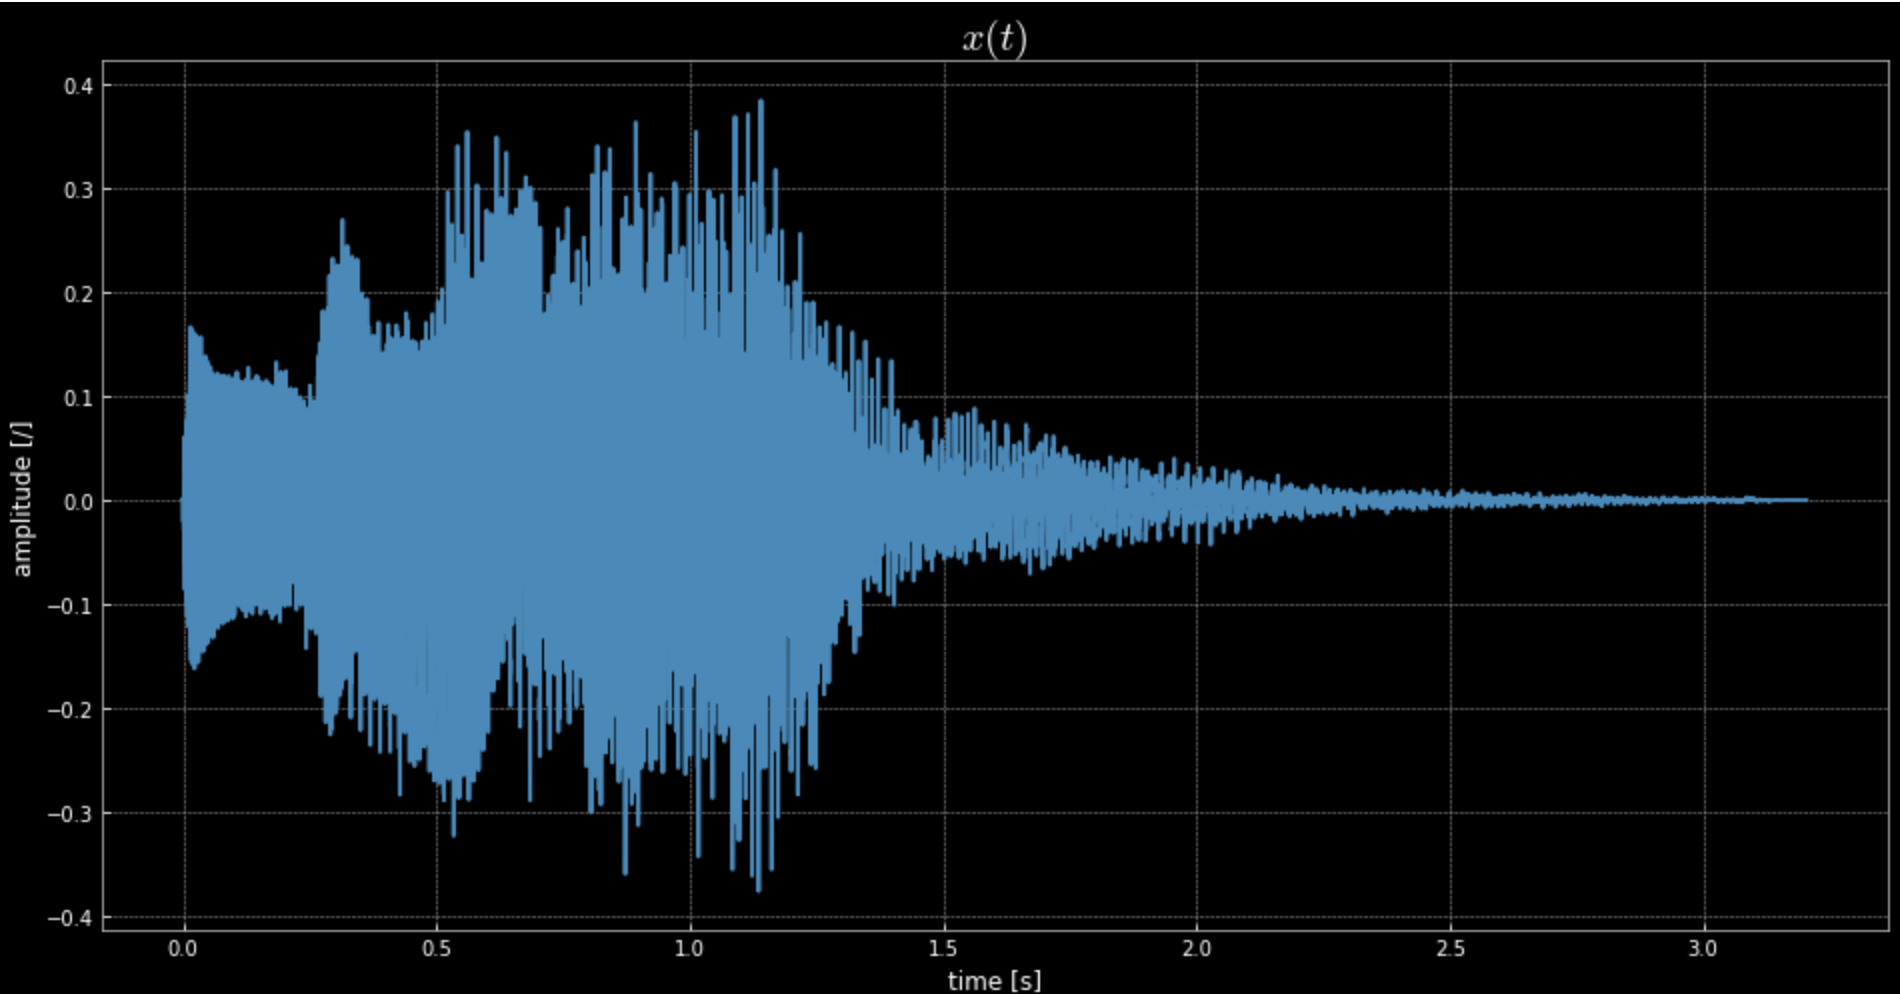
\includegraphics[width=220pt]{figs/1.png}
    \label{fig:waveform}
\end{figure}

The wave form constitutes of the amplitude  in the time domain. To analyze it in the frequency domain we use discrete fourier transform. As we want to know the frequencies over time we do fourier transform over windowed signal. The resulting graph is called a spectrogram, which represents the signal in the frequency domain.

%% Insert two spectrograms here
\begin{figure}[ht]
    \centering
    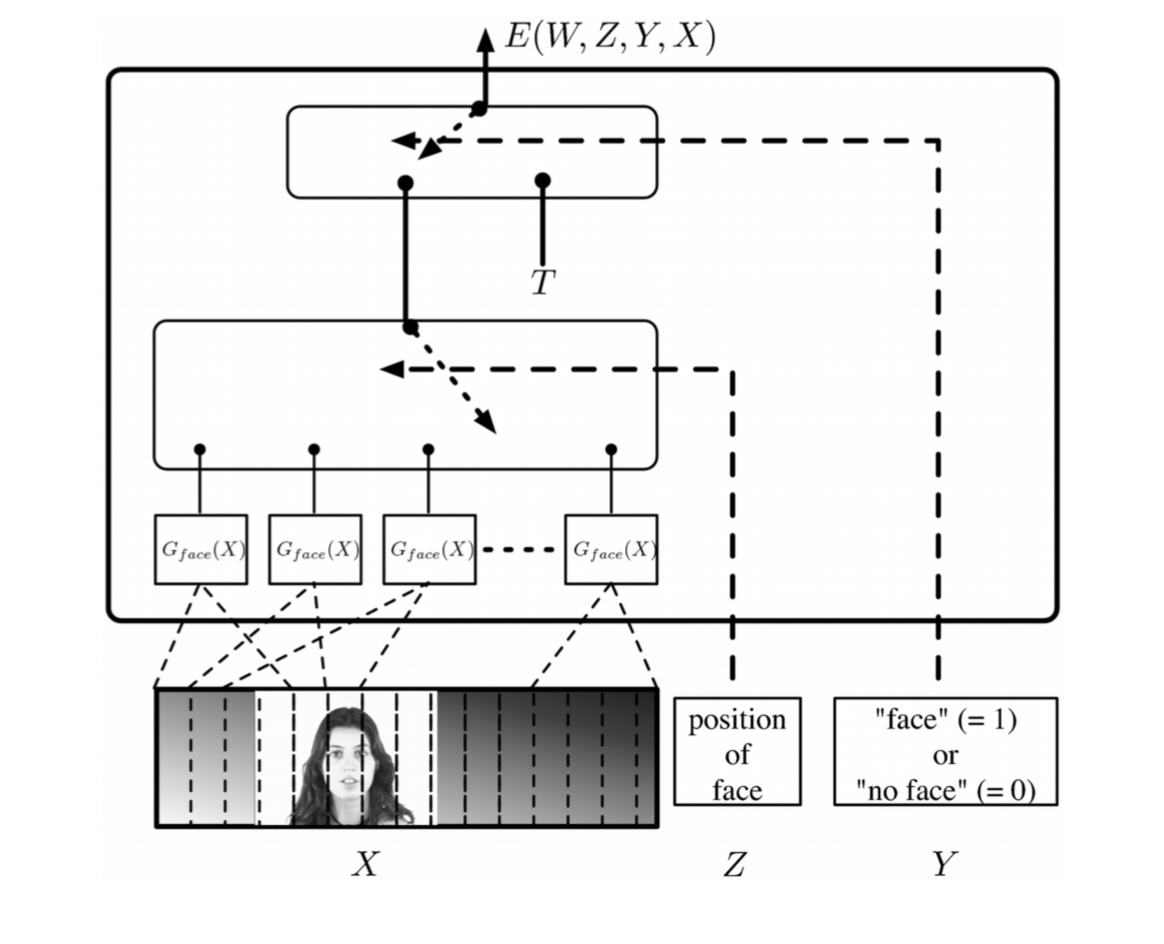
\includegraphics[width=300pt]{figs/2.png}
    \label{fig:spectrogram}
\end{figure}

The challenge is to figure out which corresponding piano keys we should play to reproduce the audio. We can either pick the frequencies from the spectrogram or we can use all frequencies of piano keys. When we do a convolution of the audio sample with this reconstructed sample we will observe that the frequencies of audio sample separated. 

In the lab we did convolution with reconstructed sample which consisted of the frequencies we guessed from spectrogram. The spectrogram of the natural signal and the one we generated can be seen below.
%% insert two spectrograms of orginal and reconstruction
\begin{figure}[ht]
    \centering
    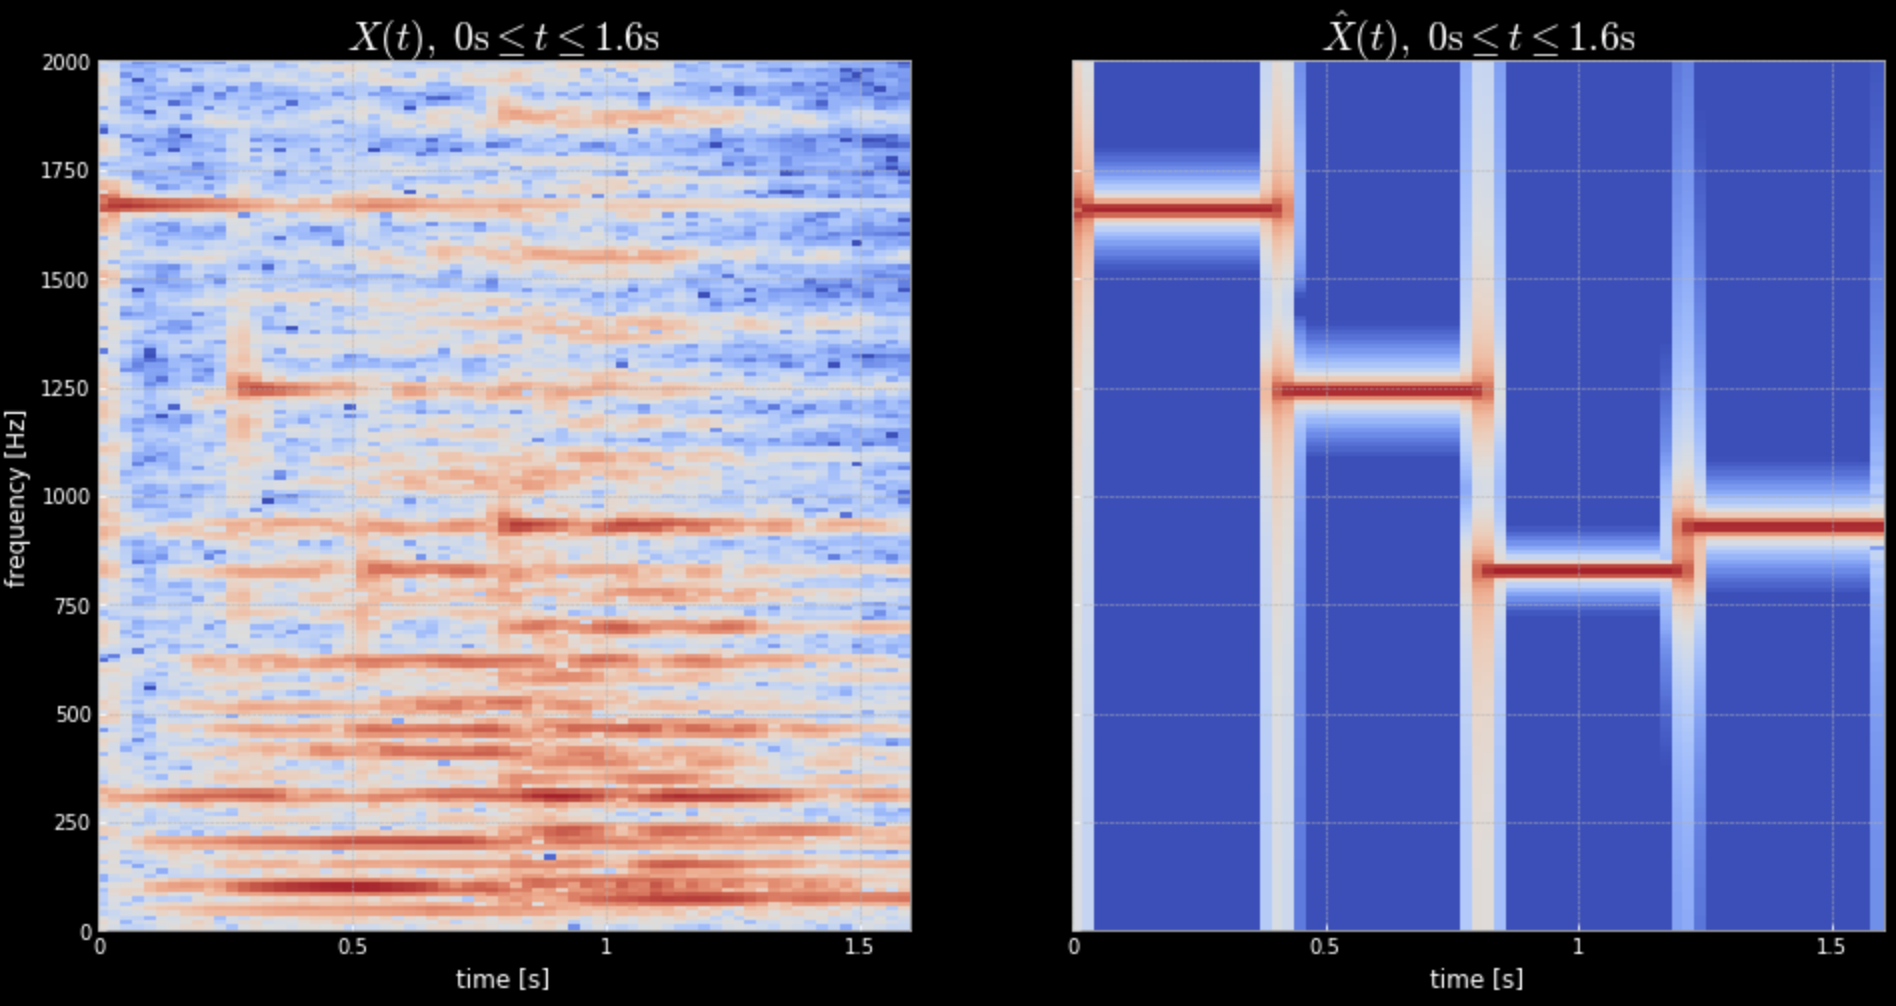
\includegraphics[width=300pt]{figs/3.png}
    \label{fig:spectrograms of original and reconstruction}
\end{figure}
